\section{Modified Keplerian Hohmann Transfer}
Since the orbits of Earth and Mars are assumed to be circular in this investigation, the lowest
maneuver cost transfer between the two bodies using Keplerian dynamics is a Hohmann transfer, shown
in \cref{fig:Hohmann}. However, this only applies if the orbits are coplanar. Hence, a plane change
maneuver must be introduced to account for the difference in the orbital planes. These inclination
change maneuvers are cheapest at apoapsis, so this is achieved by including the plane change in the
maneuver cost of the second Hohmann burn ($\Delta v_{2}$ in \cref{fig:Hohmann}) to form a modified
Hohmann transfer that serves as the baseline $\Delta v$ cost for direct patched conic transfers
between Earth and Mars.

\begin{figure}[ht]
    \centering
    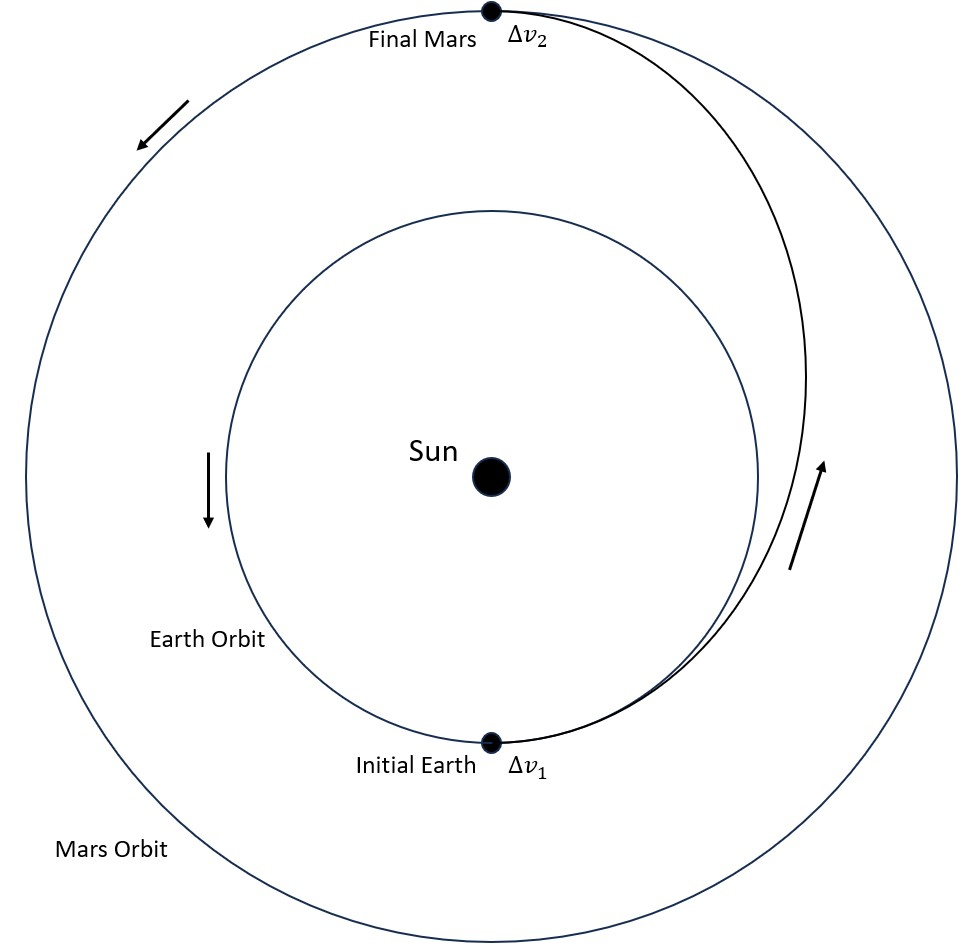
\includegraphics[width=0.5\textwidth]{figures/Hohmann.jpg}
    \caption{Hohmann transfer between Earth and Mars.}
    \label{fig:Hohmann}
\end{figure}

To serve as a baseline transfer between cislunar orbits and a Sun-Mars $L_{1}$ halo orbit for this
investigation, a Hohmann transfer between the Earth's orbit (assumed circular at a radius of
$1.49598\times10^{8}$) and the Sun-Mars $L_{1}$ distance ($2.26858\times10^{8}$) is constructed.
The following equations are used to calculate the modified Hohmann transfer combined with a plane
change:
\begin{equation}
    \Delta v_{1}=\sqrt{\frac{\mu_{2BP}}{r_{1}}}(\sqrt{\frac{2r_{2}}{r_{1}+r_{2}}}-1),
    \label{eq:Hohmann1}
\end{equation}
\begin{equation}
    \Delta v_{2}=\sqrt{v_{H}^{2}+v_{2}^{2}-2v_{H}v_{2}\cos\Delta i},
    \label{eq:Hohmann2}
\end{equation}
\begin{equation}
    v_{H}=\sqrt{\frac{\mu_{2BP}}{r_{2}}(\frac{2r_{1}}{r_{1}+r_{2}})},
    \label{eq:transferv}
\end{equation}
\begin{equation}
    v_{2}=\sqrt{\frac{\mu_{2BP}}{r_{2}}},
    \label{eq:circlev}
\end{equation}
where $\Delta v_{1}$ and $\Delta v_{2}$ are the two burns of the transfer, $\mu_{2BP}$ is the Sun's
gravitational parameter, $r_{1}$ and $r_{2}$ are the Earth's orbit and Sun-Mars $L_{1}$ radii,
respectively, $v_{H}$ is the velocity at apoapsis of the Hohmann transfer ellipse, $v_{2}$ is the
circular velocity at Sun-Mars $L_{1}$, and $\Delta i$ is the difference in inclination between the
two planes. This results in a total $\Delta v$ for the modified Hohmann transfer of $5.639$ km/s.
This value can be directly compared to the total maneuver costs of the two categories of transfers
developed in this investigation to find lower-cost transfers.

As stated previously, the minimum-cost modified Hohmann transfer has the plane change maneuver
occur at the apoapsis of the transfer ellipse. This also implies that the lowest cost MMAT
transfers occur when the second burn is located at the apoapsis of the bridge conic arc. The TOF of
the Hohmann transfer arc can be calculated analytically:
\begin{equation}
    TOF=\pi\sqrt{\frac{(r_{1}+r_{2})^{2}}{7\mu_{2BP}}},
    \label{eq:HohmannTOF}
\end{equation}
which is analogous to the times-of-flight of the MMAT bridge conic arcs. The minimum-$\Delta v$
transfer has a TOF of $258$ days.
